\section{绪论}\label{sec:introduction}

\subsection{波导缝隙天线的研究背景与意义}
    在Maxwell在宏观意义上描述了电磁现象并建立了电磁理论基础后，电磁理论与微波技术在工程领域上得到了广泛应用，时至今日，电磁波在
工业、农业、国防以及民用日常等方面都作为信息载体得到了广泛应用。天线系统作为信息传输与感知的关键前端，其性能指标日益受到关注，在众
多天线类型中，波导缝隙天线因其结构紧凑、功率容量大、辐射效率高、口径场分布易于控制等优点，在机载火控雷达、气象雷达、导航系统、导弹
制导及单脉冲跟踪雷达等领域得到了广泛应用，特别是在需要高增益、低副瓣、高指向精度的系统中，波导缝隙阵列天线展现出不可替代的优势。

    高功率微波（High-Power Microwave，HPM）技术在现代雷达、电子对抗、定向能武器及无线通信系统重扮演着日益重要的角色。作为HPM辐射系统的关键末端，高功率微波
天线的性能直接决定了整个系统的效能。HPM天线除增益、功率容量、结构紧凑性及波束扫描等特性外，副瓣电平（Sidelobe Level，SLL）也是衡量
天线抗干扰能力和能量聚焦能力的重要指标。低副瓣设计可以有效降低系统对非目标方向的辐射，减少杂波干扰，提升信号检测的可靠性。在雷达系统中，
低副瓣天线有助于抑制地杂波、海杂波及敌方干扰，提高目标识别精度；在通信系统中，则可降低邻道干扰，提升频谱利用率。当前，随着电磁环境日益
复杂，众多工程应用对天线副瓣电平提出了更高要求，典型指标已从传统设计的-20dB～-25dB向-30dB及以下迈进。

    S波段（2GHz～4GHz）因其良好的传播特性和适中的天线尺寸，广泛应用于气象雷达、航空导航、卫星通信及工业科学医疗（ISM）频段等领域。中心
频率2.45GHz尤为典型，是Wi-Fi、蓝牙、微波加热等民用技术的核心频段，同时也是某些雷达系统的工作频率。然而，目前国内外关于波导缝隙阵列天线
的研究多集中于X波段、Ku波段及以上频段，针对S波段、特别是副瓣电平优于-30dB的高性能波导缝隙阵列天线的系统研究相对较少。S波段波长较长（约122mm），
天线尺寸较大，缝隙间互耦效应复杂，加工与调试难度也相应增加，这使得在S波段实现低副瓣设计具有独特的理论价值与工程挑战。

    因此，开展S波段、中心频率2.45GHz、副瓣电平低于-30dB的波导缝隙阵列天线设计研究，不仅能够填补该频段低副瓣波导缝隙天线的技术空白，也为
后续工程应用提供了可参考的设计方法与实现路径，具有重要的理论意义与工程实用价值。

\subsection{波导缝隙天线的历史与发展现状}

\subsubsection{国外研究现状}
    波导缝隙天线的理论研究可追溯至20世纪40年代。1948年，Stevenson首次引入等效传输线理论，推导了波导宽面纵向缝隙的归一化谐振电导计算公式，
奠定了波导缝隙天线分析的基础\supercite{1}。此后，Oliner于1959年利用变分法同时求解了缝隙导纳的实部与虚部，并考虑了波导壁厚对谐振长
度的影响\supercite{2}。Yee在1974年进一步完善了谐振长度与缝隙偏置之间的数值关系，使设计更加精确\supercite{3}。

    20世纪70年代末至80年代，Elliott提出了著名的三个设计方程，综合考虑了缝隙内外部互耦、高次模影响以及口径场分布，成为现代波导缝隙阵列天线
设计的主流方法\supercite{4}\supercite{5}。此后，Sangster、Gulick等学者分别在矩量法分析、高精度综合方法等方面做出了重要贡献。
    近年来，国外学者在波导缝隙天线的高增益、低副瓣、和差波束及宽带化等方面取得了诸多进展。例如，Bernal等人设计了工作于2.3GHz的高功率窄带波
导缝隙阵列，如图1.1所示，增益达30dB，用于远程引爆系统\supercite{6}；
\begin{figure}[htb!]
    \centering
    \begin{subfigure}{.5\textwidth}
        \centering
        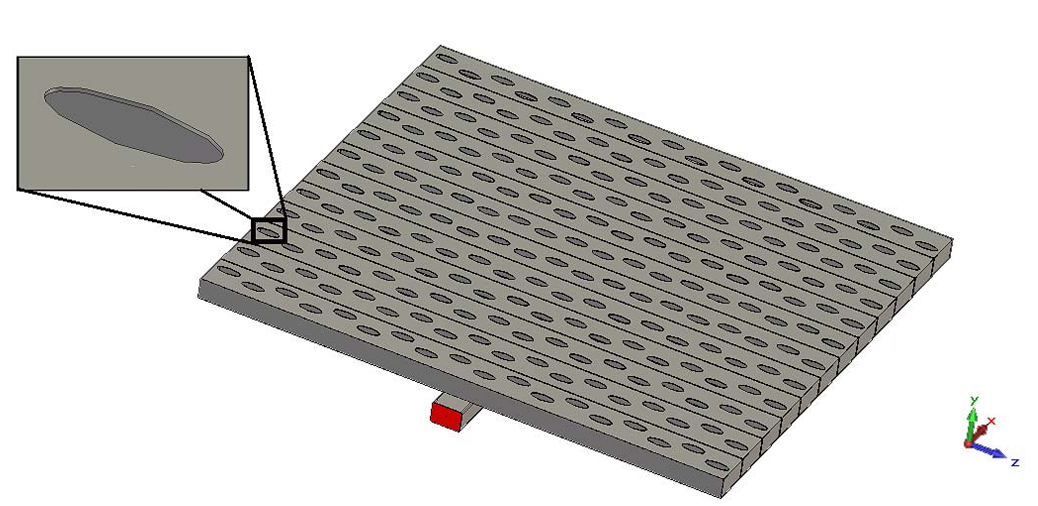
\includegraphics[height=.15\textheight]{./img/参考文献6a.png}
        \caption{辐射体结构模型}
        \label{fig_ref_6a}
    \end{subfigure}
    \begin{subfigure}{.35\textwidth}
        \centering
        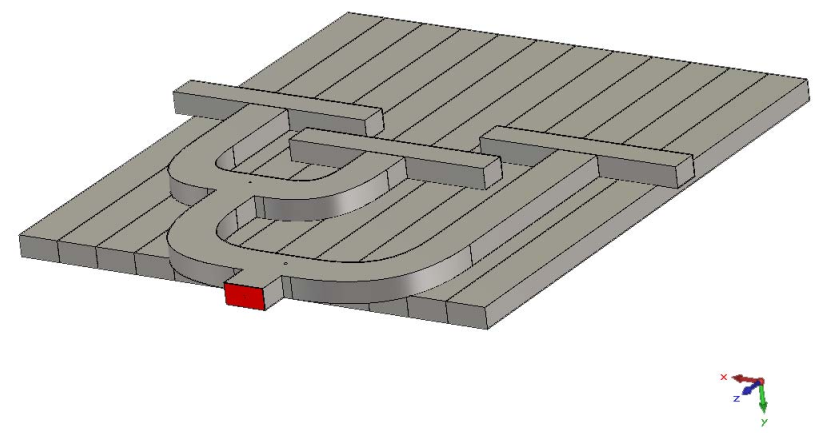
\includegraphics[height=.15\textheight]{./img/参考文献6b.png}
        \caption{馈电层模型}
        \label{fig_ref_6b}
    \end{subfigure}
    \caption{高功率窄带波导缝隙阵列}
    \label{fig_ref_6}
\end{figure}
    
    Gatti等人实现了Ku波段双极化波导缝隙阵列，如图1.2所示，副瓣电平控制在-25dB以下\supercite{7}；
\begin{figure}[htb!]
    \centering
    \begin{subfigure}{.8\textwidth}
        \centering
        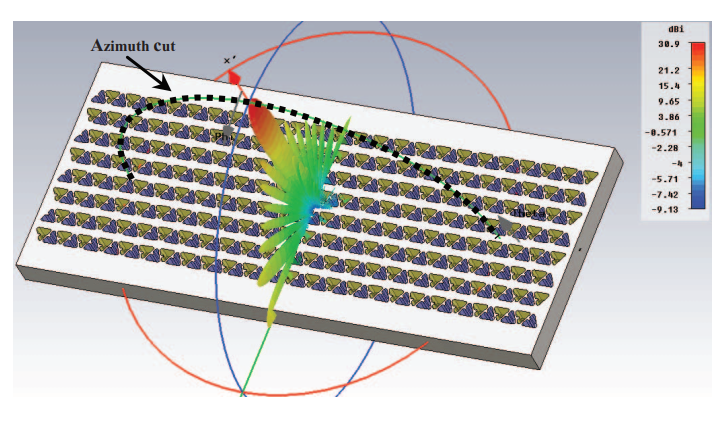
\includegraphics[height=.3\textheight]{./img/参考文献7a.png}
        \caption{三维辐射图}
        \label{fig_ref_7a}
    \end{subfigure}
    \newline
    \begin{subfigure}{.8\textwidth}
        \centering
        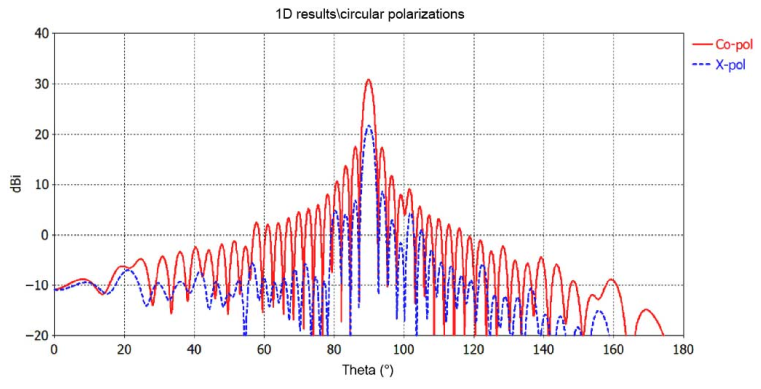
\includegraphics[height=.3\textheight]{./img/参考文献7b.png}
        \caption{方位角辐射图}
        \label{fig_ref_7b}
    \end{subfigure}
    \caption{Ku波段双极化波导缝隙阵列}
    \label{fig_ref_7}
\end{figure}

    Costa等人设计了毫米波段三频带波导缝隙线阵\supercite{8}，如图1.3所示，在低副瓣实现方面，Dolph-Chebyshev综合法、Taylor综合法被广泛应用于阵列激励幅度的优化设计，结合有源导纳法，可在设计
阶段有效抑制副瓣电平。
\begin{figure}[htb!]
    \centering  
    \begin{subfigure}{.35\textwidth}
        \centering
        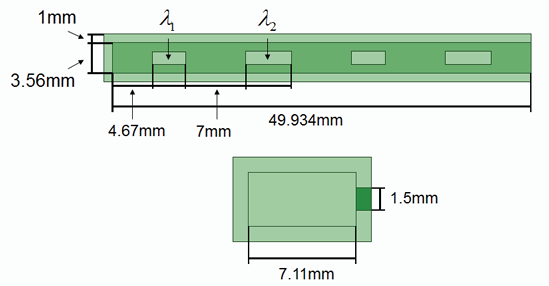
\includegraphics[height=.15\textheight]{./img/参考文献8a.png}
        \caption{仿真模型图}
        \label{fig_ref_8a}
    \end{subfigure}
    \begin{subfigure}{.35\textwidth}
        \centering
        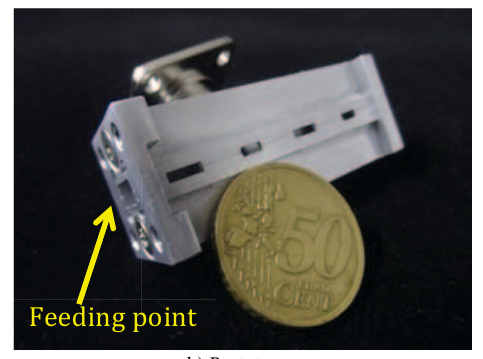
\includegraphics[height=.15\textheight]{./img/参考文献8b.png}
        \caption{实物模型图}
        \label{fig_ref_8b}
    \end{subfigure}
    \caption{毫米波段三频带波导缝隙线阵}
    \label{fig_ref_8}
\end{figure}

    总体来看，国外在X波段及以上频段的波导缝隙阵列天线研究已相当成熟，但在S波段、尤其是不低于-30dB的低副瓣设计方面，公开文献相对较少，相关设
计方法与工程经验仍有待系统化。

\subsubsection{国内研究现状}
    国内对波导缝隙天线的研究起步较晚，早期以实验测量和工程经验为主。进入90年代后，随着计算机技术与电磁场数值方法的发展，矩量法、有限元法（FEM）、
时域有限差分法（FDTD）等被逐步引入波导缝隙天线的分析与综合中，设计精度显著提高。

    谢艳萍\supercite{9}设计了C波段高增益水平极化波导缝隙全向天线，如图1.4所示，采用四块铝片组装波导以降低成本，通过遗传算法优化馈电探针，在5.6GHz～5.85GHz频带内实现VSWR<1.5，
最大增益约13.99dBi，不圆度控制在±1.5dB以内。该工作在波导结构改进和探针馈电优化方面具有较好的参考价值。
\begin{figure}[htb!]
    \centering
    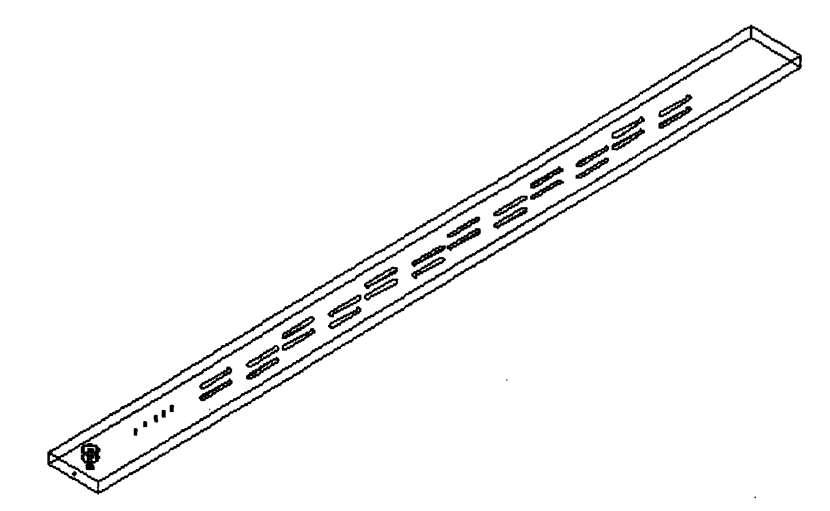
\includegraphics[height=.3\textheight]{./img/参考文献9.png}
        \caption{天线结构模型}
        \label{fig_ref_9}
\end{figure}

    王竣\supercite{10}设计了X波段高增益低副瓣波导缝隙阵列天线，如图1.5所示，应用Dolph-Chebyshev综合法分别对波导线阵的缝隙偏移量和耦合波导的斜缝倾角进行优化，实现了副瓣电平低于
-30dB（H面）和-17dB（E面），并设计了和差馈电网络，验证了天线的单脉冲性能。该研究系统展示了低副瓣波导缝隙阵列从理论综合到仿真、加工、测试的完整流程。
\begin{figure}[htb!]
    \centering
    \begin{subfigure}{.5\textwidth}
        \centering
        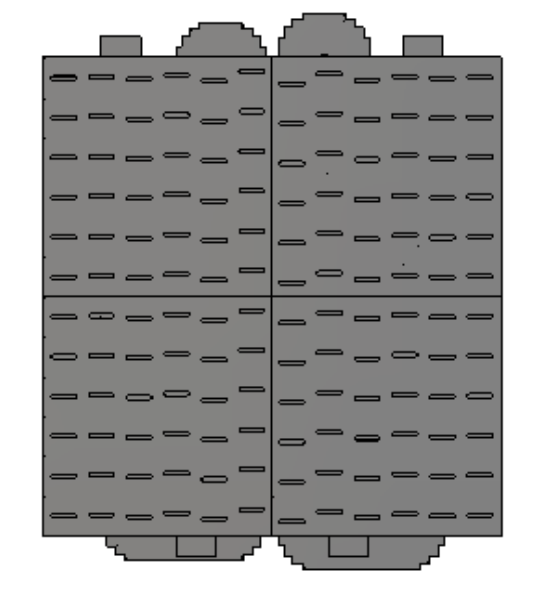
\includegraphics[height=.2\textheight]{./img/参考文献10a.png}
        \caption{仿真模型图}
        \label{fig_ref_10a}
    \end{subfigure}
    \begin{subfigure}{.5\textwidth}
        \centering
        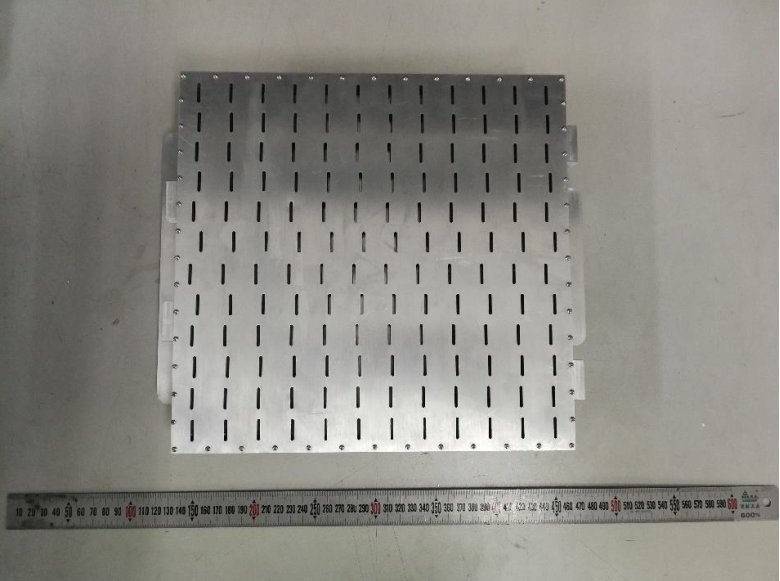
\includegraphics[height=.2\textheight]{./img/参考文献10b.png}
        \caption{实物模型图}
        \label{fig_ref_10b}
    \end{subfigure}
    \caption{X波段高增益低副瓣波导缝隙阵列天线}
    \label{fig_ref_10}
\end{figure}

    侯万杉\supercite{11}等人针对高功率微波应用中的波导缝隙阵天线，提出了一种考虑缝隙互耦效应的电导函数提取新方法。该方法利用现代计算机技术快速计算缝隙电导函数，避免了
复杂的理论推导与迭代运算。基于该方法设计的S波段（中心频率2.458GHz）波导缝隙面阵，在输入端采用了与目标馈电幅度比一致的提取策略，使得各端口反射系数范围降至-37.2dB～-27.7dB，相
比传统Stevenson公式设计方法至少降低了19dB，同时实现了-30.2dB的低副瓣电平和332.6MW的高功率容量。该研究对S波段低副瓣波导缝隙
天线的工程设计具有重要的指导意义。
\begin{figure}[htb!]
    \centering
    \begin{subfigure}{.6\textwidth}
        \centering
        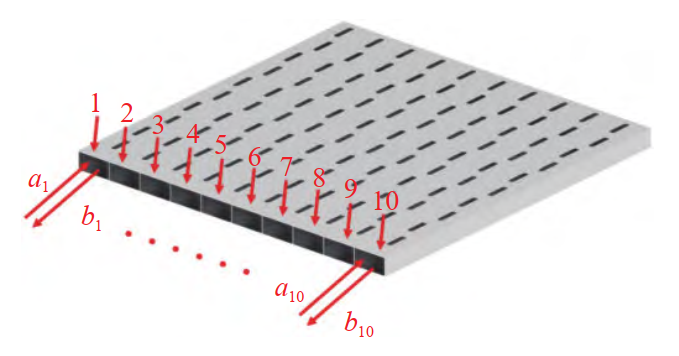
\includegraphics[height=.3\textheight]{./img/参考文献11a.png}
        \caption{仿真模型图}
        \label{fig_ref_11a}
    \end{subfigure}
    \newline
    \begin{subfigure}{.45\textwidth}
        \centering
        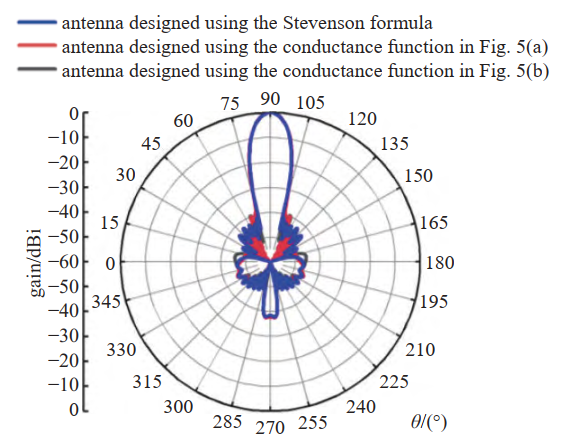
\includegraphics[height=.3\textheight]{./img/参考文献11b.png}
        \caption{E面辐射图}
        \label{fig_ref_11b}
    \end{subfigure}
    \begin{subfigure}{.45\textwidth}
        \centering
        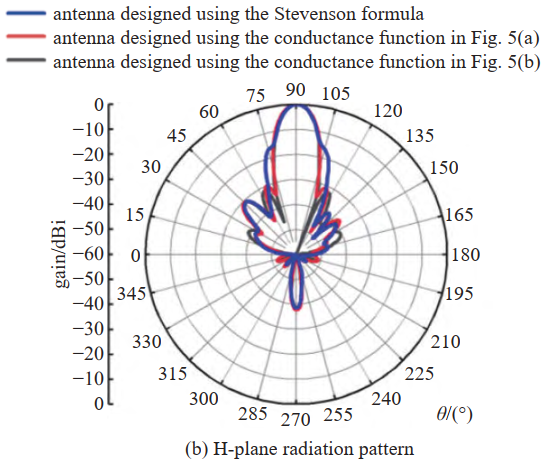
\includegraphics[height=.3\textheight]{./img/参考文献11c.png}
        \caption{H面辐射图}
        \label{fig_ref_11c}
    \end{subfigure}
    \caption{S波段低副瓣波导缝隙面阵}
    \label{fig_ref_11}
\end{figure}

    邓世露\supercite{12}围绕低副瓣波导缝隙阵列天线开展了系统研究，分别设计了矩形波导、单脊波导和基片集成波导（SIW）三种形式的天线。在X波段，设计了低副瓣矩形波导缝隙行
波阵列天线，通过相邻波导镜像倒置有效抑制了交叉极化；进一步设计了单脊波导缝隙行波阵列天线，通过增加缝隙宽度、调整缝隙间距和优化导纳分布，在9.05GHz～9.75GHz频带内实现副瓣低于-30
dB、增益大于28dBi、带宽达700MHz；在此基础上，设计了双极化波导缝隙行波阵列天线，在两种极化方式下均实现副瓣低于-30dB、增益大于31dBi，且波束指向和波束宽度高度一致。在Ka波段，
设计了基于SIW的低副瓣缝隙驻波阵列天线，并通过稀疏化处理和复合超表面加载，将带宽增加600MHz、增益提高1dBi、副瓣降低2dB，最终加工测试验证了设计的有效性。该研究覆盖了行波阵与驻
波阵两种天线形式，工作频段涵盖X波段和Ka波段，对低副瓣波导缝隙天线的多样化设计具有较好的参考价值。
\begin{figure}[htb!]
    \centering
    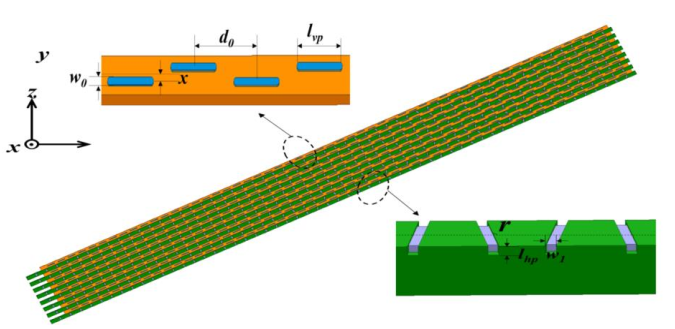
\includegraphics[width=.9\textwidth]{./img/参考文献12.png}
    \caption{邓世露设计的波导缝隙阵列天线}
    \label{fig_ref_12}
\end{figure}


    此外，国内学者在基片集成波导（Substrate Integrated Waveguide, SIW）缝隙天线、宽带波导缝隙阵列、共形波导缝隙天线等方面也开展了大量研究。例如，胡伟\supercite{13}等人设计了X波段宽带波导缝隙阵列，史嘉\supercite{14}等人设计了新型X波段波导
缝隙阵列等。但在S波段，公开报道的低副瓣（< -30dB）波导缝隙阵列天线研究仍较为有限，侯万杉\supercite{11}等人的工作是该频段内具有代表性的研究成果之一。

\subsubsection{国内外文献综述简析}
    通过对国内外研究现状的调查与分析，并对现有天线dd设计方法以及优缺点进行对比与分析，结果表明，低副瓣的实现、高功率容量一直是波导缝隙阵列天线设计领域中的热点问题。总体设计方法已趋于成熟：即以Elliott\supercite{4}\supercite{5}
的三个设计方程为基础，结合Dolph-Chebyshev综合法、Taylor综合法等优化激励幅度分布，并通过有源导纳法及电磁仿真软件（HFSS、CST等）进行波导缝隙阵列天线的仿真设计。

    现有研究成果主要集中在X波段、Ku波段以及毫米波频段，在S波段的研究相对较少，尤其是副瓣电平优于-30dB的高性能波导缝隙阵列天线的系统研究更为有限。副瓣电平低于-30dB的设计对激励幅度精度、缝隙间互耦补偿等方面有着更高的要求。而S波段
波长较长，天线尺寸较大，缝隙间互耦效应复杂，加工与调试难度也相应增加，这使得在S波段实现低副瓣设计具有独特的理论价值与工程挑战。

    一般来说主要由一下三种方法来实现天线的低副瓣性能：第一，使用经典二项式分布确定各阵元馈电幅度\supercite{16}\supercite{17}，可以实现无副瓣电平，但主瓣宽度较大；第二，应用Dolph-Chebyshev\supercite{18}\supercite{19}\supercite{20}\supercite{21}综合法
求解阵元激励分布，可以在给定副瓣电平内实现主瓣最窄；第三，应用Taylor\supercite{22}\supercite{23}\supercite{24}综合法求解各阵元激励分布，可以实现临近主瓣的副瓣电平相等，其余副瓣依次降低的特性。本课题分别针对Dolph-Chebyshev综合法和Taylor综
合法进行优化设计，实现天线的低副瓣特性。

\subsection{本课题的研究内容及论文结构}
    本课题以S波段中心频率2.45GHz为应用背景，根据系统对天线高增益、低副瓣的性能需求，研究利用波导缝隙阵列实现低副瓣天线的设计方法。预计论文工作包含以下内容：
    
    （1）绪论

    介绍课题来源、背景。通过查阅国内外文献，了解国内外在该方向上的发展进程以及研究成果，并对国内外研究成果进行总结，梳理全文内容与章节。

    （2）波导缝隙阵列天线基本理论

    介绍波导缝隙阵列天线的基本理论。由矩形波导缝隙天线引入波导缝隙天线的辐射原理，推导各种形式缝隙的等效阻抗或导纳；分析缝隙间互耦。讨论可以实现高增益低副瓣的
设计方法，如Dolph-Chebyshev综合法和Taylor综合法。

    （3）波导缝隙线阵设计

    以S波段中心频率2.45GHz为设计目标，进行线阵的优化仿真，在中心频率固定即波导尺寸固定的情况下，通过对缝隙位置和数量的调整，在保证方向图不失真的前提下，尽量降低副瓣电平，
以便后续面阵设计时有更大的设计空间。仿真分析不同参数对天线性能的影响，并优化天线结构，验证设计方法的有效性。

    （4）波导缝隙面阵设计

    在优化的线阵基础上，设计面阵天线，并进行仿真分析，验证设计方法的有效性。

    （5）总结与展望

    总结全文工作，分析研究中存在的不足，并对未来的研究方向进行展望。

\section{波导缝隙天线基本理论}

\subsection{引言}

    本章主要介绍与波导o缝隙阵列天线相关的基本理论，包括矩形波导缝隙天线的辐射原理、各种形式缝隙的等效阻抗或导纳的推导，以及缝隙间互耦的分析。最后，讨论实现高增益低副瓣设计
的方法，如Dolph-Chebyshev综合法和Taylor综合法。以上理论在本课题天线设计的过程中起到了很重要的作用。

\subsection{矩形波导缝隙天线}

    矩形波导（如图2.1所示）是波导缝隙天线最常用的传输线形式。
    
\begin{figure}[htb!]
    \centering
    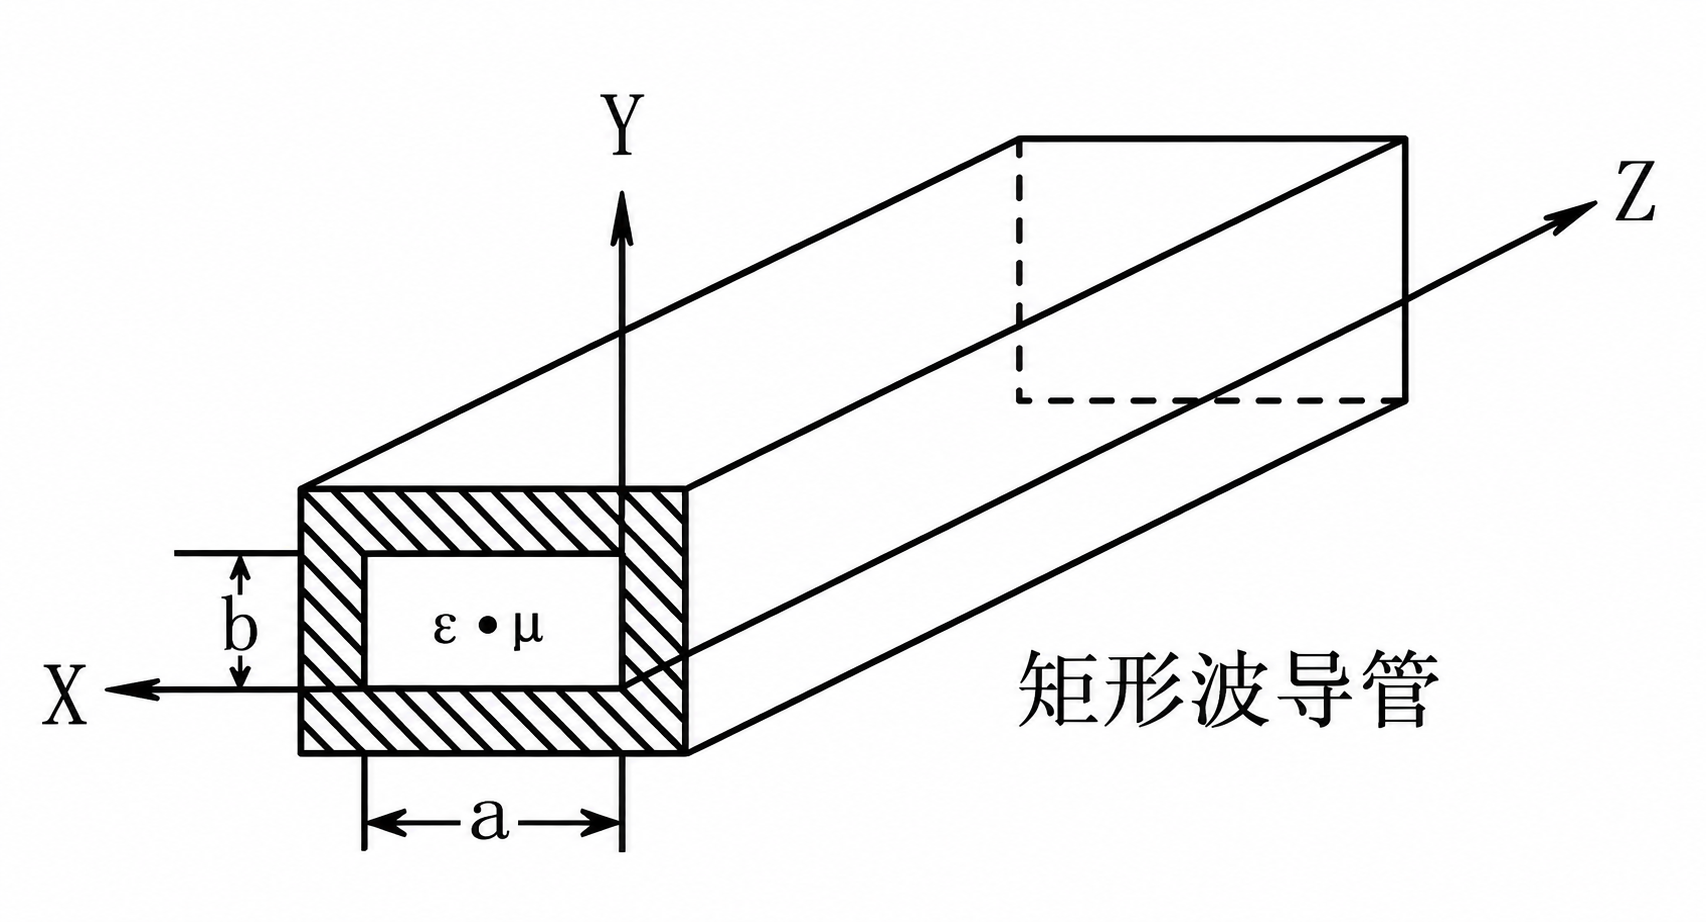
\includegraphics[height=.3\textheight]{./img/原理2.1.1.png}
    \caption{矩形波导示意图}
    \label{fig_principle_2.1.1}
\end{figure}

    对TM模（$H_z$=0,$E_0$决定于激励情况）
\begin{equation}
    \begin{cases}
        H_{x0}=j\frac{\omega \varepsilon}{k_c^2}E_0
            \left(\frac{n\pi}{b}\right)
            \sin\left(\frac{m\pi}{a}x\right)
            \cos\left(\frac{n\pi}{b}y\right)\\
        H_{y0}=-j\frac{\omega \varepsilon}{k_c^2}E_0
            \left(\frac{m\pi}{a}\right)
            \cos\left(\frac{m\pi}{a}x\right)
            \sin\left(\frac{n\pi}{b}y\right)\\
        E_{x0}=-j\frac{\beta}{k_c^2}E_0
            \left(\frac{m\pi}{a}\right) 
            \cos\left(\frac{m\pi}{a}x\right)
            \sin\left(\frac{n\pi}{b}y\right)\\
        E_{y0}=-j\frac{\beta}{k_c^2}E_0
            \left(\frac{n\pi}{b}\right)
            \sin\left(\frac{m\pi}{a}x\right)
            \cos\left(\frac{n\pi}{b}y\right)\\
    \end{cases}
\end{equation}

    对TE模（$E_z$=0,$E_0$决定于激励情况）
\begin{equation}
    \begin{cases}
        E_{x0}=j\frac{\omega \mu}{k_c^2}H_0
            \left(\frac{n\pi}{b}\right)
            \cos\left(\frac{m\pi}{a}x\right)
            \sin\left(\frac{n\pi}{b}y\right)\\
        E_{y0}=-j\frac{\omega \mu}{k_c^2}H_0
            \left(\frac{m\pi}{a}\right)
            \sin\left(\frac{m\pi}{a}x\right)
            \cos\left(\frac{n\pi}{b}y\right)\\
        H_{x0}=j\frac{\beta}{k_c^2}H_0
            \left(\frac{m\pi}{a}\right)
            \sin\left(\frac{m\pi}{a}x\right)
            \cos\left(\frac{n\pi}{b}y\right)\\
        H_{y0}=j\frac{\beta}{k_c^2}H_0
            \left(\frac{n\pi}{b}\right)
            \cos\left(\frac{m\pi}{a}x\right)
            \sin\left(\frac{n\pi}{b}y\right)\\
    \end{cases}
\end{equation}

    假如波向 z 方向传播，故各个场分量的复振幅求得后，均乘以n相位因子$e^j{bete}z$,即得矩形波导的TE模场强。

    矩形波导主模为TE$_{10}$模，图2.2为其各个面上的电磁场，当矩形波导仅传输主模时，可以等效为双线传输线，波导内部的电磁场分布具有明确的规律：电场主要集中在波导宽边的中心区域，
并沿宽边方向呈正弦分布；磁场则同时具有横向和纵向分量。内部电磁场表达式如下：

\begin{figure}[htb!]
    \centering
    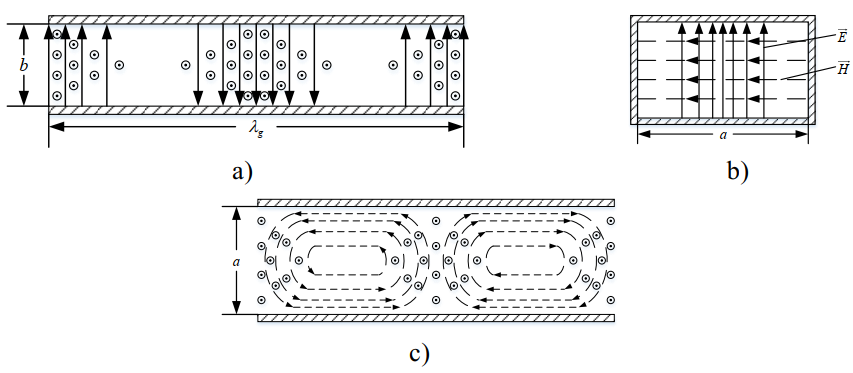
\includegraphics[height=.3\textheight]{./img/原理2.1.2.png}
    \caption{TE$_{10}$波的电磁场分布与面电流分布}
    \label{fig_principle_2.2}
\end{figure}

\begin{equation}    
    \begin{aligned}
        \vec{E}_t &= \vec{E}_{10t} \exp(\mp j \beta_{10}z) \\
        \vec{H}_t &= \pm \vec{H}_{10t} \exp(\mp j \beta_{10}z)\\
        \vec{H}_t &= j \vec{H}_{10z} \exp(\mp j \beta_{10}z)
    \end{aligned}
\end{equation}
其中，$\vec{E}_t$和$\vec{H}_t$分别为横向电场和磁场分量，$\vec{H}_{10z}$为纵向磁场分量，$\beta_{10}$为TE$_{10}$模的传播常数。根据电磁场边界条件，波导内壁的表面电流密度由磁场切向分量决定，其流向与磁场方向满足右手定则。

    波导作为一种封闭的金属结构，能够对内部传播的电磁波形成有效屏蔽。当将矩形波导近似视为理想导体时，其内部体电场为零，波导内壁成为一个等位面。在此条件下，波导内部传播的电磁波会在其金属壁面上激励出感应电流。由于趋肤效应的影响，这些感应电流主要集中在波导的内壁表面流动。
波导内壁上的面电流密度分布直接由壁面处的切向磁场决定.设波导内壁的单位法向向量为$\vec{n}$，则表面电流密度$\vec{J}_s$与切线磁场$\vec{H}_t$之间的关系可通过边界条件表示为：

\begin{equation}
    \vec{J}_s = \vec{n} \times \vec{H}_t
\end{equation}
    
    该式表明，内壁上的电流密度大小与切向磁场强度成正比，方向则同时垂直于法向与磁场方向。

    将一根波导放至自由空间，在波导输入端输入信号，波导终端接短路版。
当在矩形波导宽壁上偏离中心轴线一定距离处开设一条纵向缝隙时，该缝隙会
对波导宽壁上的横向传导电流产生截断效应。缝隙口面处的传导电流将转化为
位移电流，从而激励电磁波向外辐射；与此同时，缝隙也会激发若干高次模式，
这些模式会向前后两个方向传播。由于波导结构中高次模的截止特性，这些模式
在传播很短的距离后便迅速衰减，最终可忽略不计。缝隙偏离波导中心的距离以
及缝隙本身的长度，共同决定了其对原传导电流的截断强度与相位关系，进而控
制了缝隙口面上电场分布的幅值与相位。这些参数最终影响了天线的远场辐射
方向图以及输入端口的阻抗特性。

\subsection{波导缝隙天线辐射原理}

\subsubsection{理想缝隙天线}
    理想缝隙天线是一种基础的天线分析模型，其构造非常简单：在一块理想导体平板上开设一条细窄的缝隙，且该平板被视为面积无限大、厚度无限薄。如图2.1 a)所示，该缝隙的长度$L$远小于工作波长$\lambda$，且缝隙宽度$w$远小于$L$。当在缝隙两端市价射频激励电压
$U_0$时，缝隙口面上会建立起电场分布$E_a$，这种结构被称作短缝隙。图2.1 b)则给出了与之互补的带状短波振子结构。
\begin{figure}[htb!]
    \centering
    \begin{subfigure}{.45\textwidth}
        \centering
        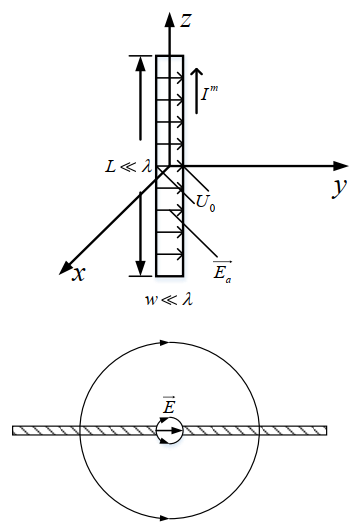
\includegraphics[height=.4\textheight]{./img/原理2.2.1a.png}
        \caption{短缝隙}
        \label{fig_principle_2.2.1a}
    \end{subfigure}
    \begin{subfigure}{.45\textwidth}
        \centering
        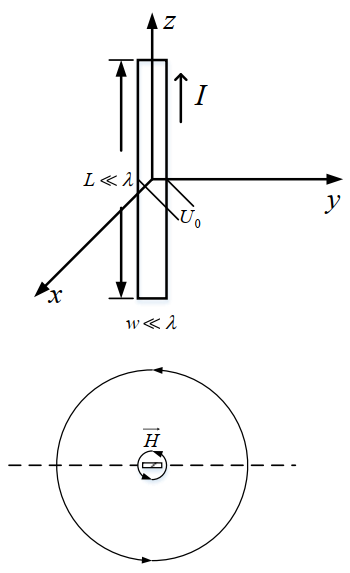
\includegraphics[height=.4\textheight]{./img/原理2.2.1b.png}
        \caption{短振子}
        \label{fig_principle_2.2.1b}
    \end{subfigure}
    \caption{短缝隙与互补短振子结构示意图}
    \label{fig_principle_2.2.1}
\end{figure}

    一个纵向长度被无线压缩的，半径为$a$≈$w$/4的圆柱短振子，可以视作一个带状短电i振子的替代结构。在结构g中$z$轴存在一定电流通过，电流最大值$I_0$
位于结构中心处，且电流分布近似为半正弦分布。根据互补原理，短缝隙与短振子在相同位置处具有相同的电场分布，因此可以通过分析短振子的电流分布来推导短缝隙的电磁分布如式2.3:

\begin{equation}
    \begin{cases} 
        E_d = j\eta \frac{kI_0L}{8\pi r} \sin\theta e^{-ikr} \\
        H_d = j\frac{kI_0L}{8\pi r} \sin\theta e^{-ikr}
    \end{cases}
\end{equation}

    因此如果存在一个相同结构的导磁片，可以求解出其磁流源辐射场：
\begin{equation}
    \begin{cases}
        H_m = j \frac{kI_0^m L}{8\pi r\eta} \sin \theta e^{-ikr}\\
        E_m = -j \frac{kI_0^m L}{8\pi r} \sin \theta e^{-ikr}
    \end{cases}
\end{equation}
    如果存在一对短缝隙天线，且为互补的，可以求解其上感应电流空间场：
\begin{equation}
    \begin{cases}
        E_s = -E_e^s = j \frac{kI_0^m L}{8\pi r} \sin \theta e^{-ikr} \\
        H_s = -H_e^s = -j \frac{kI_0^m L}{8\pi r\eta} \sin \theta e^{-ikr}
    \end{cases}
\end{equation}
    式中，带有下标$s$的物理量代表短缝隙天线自身的相关参数。由此可以得出，位于面$s$上的感应电流为短缝隙提供了辐射场，并且该辐射场在数值上可视为与磁流
    $I_0^m$在短缝隙平行方向上的辐射场相等。短缝隙两端所施加的电压$U_0$的大小直接决定了磁流$I_0^m$的幅值。如图2.1 b)所示，在振子结构的中点处，电流达到最大值$I_0$，
    该电流与该点表面处磁场$H_0$之间存在如下关系：
\begin{equation}
    I_0 = \oint_l \vec{H}_0 \cdot d\vec{l} = 2H_0 W
\end{equation}
因此可对其求对偶：
\begin{equation}
    I_0^m=2E_0 w=2U_0
\end{equation}

    同理，通过加与缝隙两端的射频h电压$U_0$求出其表面磁场，也可证明上述结论。综上所述，短缝隙天线的辐射原理可以通过互补原理与短振子结构进行分析和理解。
短缝隙天线的电场分布与短振子的电流分布相同，并且其辐射场可以视为由磁流源产生的辐射场。这些基本理论为后续波导缝隙阵列天线的设计提供了重要的基础。

\subsubsection{缝隙形式及其等效电路}

    波导结构本身对内部电磁场具有封闭约束作用。当在波导的金属壁面上加工出不同形式的缝隙时，这些缝隙便能够借助波导内部原有的场分布实现能量向外耦合。主模TE$_{10}$模式下
的壁电流可分解为横向和纵向两个分量。其中，横向电流沿波导宽边呈余弦规律变化，在宽边中心处幅值最大；而在波导窄边上，仅存在横向电流，且其分布较为均匀。当所开缝隙的方向与
电流线方向呈现一定夹角时，电流路径会被缝隙截断，原有的传导电流转变为位移电流继续维持流动，从而使缝隙获得激励。由此可见，波导内部传输的功率正是通过缝隙向外辐射的。
    
    如图2.4所示,是矩形波导中几种常见的开缝形式，“1”为宽边纵缝，“2”为宽边斜缝，“3”为宽边中心斜缝，“4”为宽边斜缝，“5”，“6”为窄边斜缝。根据缝隙天线的理论可得，如果缝隙切割的电流越强，那么通过缝隙产生的辐射就
越强。所以当电场保持恒定时，横向缝隙与电场相互垂直，产生的辐射能量比倾斜缝隙大；当缝隙保持固定时，电场被缝隙切割越强，从缝隙处向外辐射的能量越大。

\begin{figure}[htb!]
    \centering
        \centering
        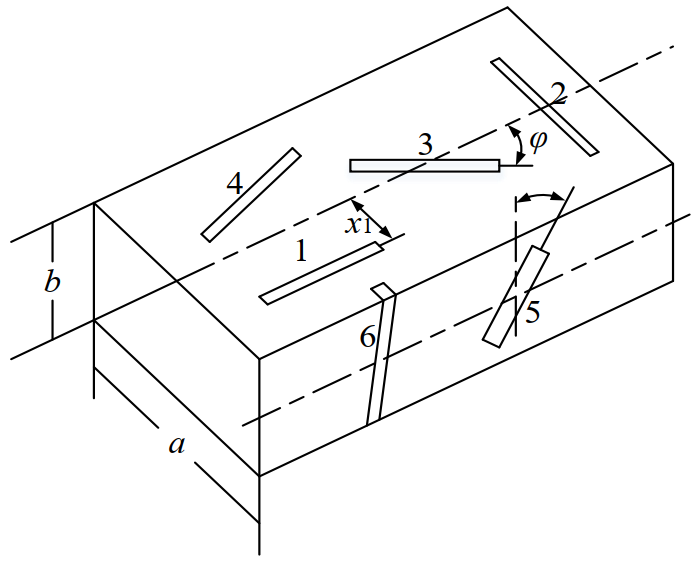
\includegraphics[height=.3\textheight]{./img/原理2.2.2.png}
        \caption{各种缝隙形式}
        \label{fig_principle_2.2.2}
\end{figure}

    通常来说，矩形波导的缝隙位置在波导的宽边波壁和窄边波壁上。 此时波导上的电流分布会随着缝隙与电流方向之间形成的夹角而发生变化。 由于横向缝隙和纵向缝隙对电流作用不同， 其等效电路和分析方法不同，
因此需要分别进行分析。

    在图2.5 a）中，当当沿波导宽边方向开设一条纵向缝隙时，缝隙两端的电流路径被截断并改变流向。此时，该纵向缝隙在等效电路中可视为一个并联导纳。在图2.5 b）中，同样在宽边上开设一条横向缝隙，该横向缝隙会切断纵向电流，
同时引起电场分布的改变。总电场$E_y$的变化导致电压发生变化，这一效应可等效为串联电路中引入一个阻抗。图2.5 c）至图2.5 e）则分别展示了宽边中心斜缝、宽边斜缝和窄边斜缝的等效电路示意图。不同形式的缝隙会对电流路径和
电场分布产生不同程度的影响，从而导致其等效电路中的导纳或阻抗参数发生变化。这些等效电路模型为分析和设计波导缝隙天线提供了重要的工具。展示了其他几种缝隙取向所对应的阻抗等效形式。在图2.5 e）中，纵向电流沿传播方向的变化与电场$E_y$
的变化，共同等效为并联电路中增加一个导纳、串联电路中增加一个阻抗的复合影响。

    对于上述各类缝隙结构，其电导或电阻的计算思路是：首先确定缝隙在两个方向上的散射场分布，然后依据功率守恒关系建立方程，进而求得相应的电阻或电导值。不过，这一计算过程可以通过更为简洁的方法实现。下面以宽边纵向缝隙为例，给出具体的推导过程。

    设$P_i$为入射功率，$P_s$为纵向缝隙的辐射功率，根据图2.5 a）中对等效电路的求解：
\begin{equation}
    \frac{1}{2} U^2 g Y_0 = P_s
\end{equation}
\begin{equation}
    \frac{1}{2} U^2 Y_0 = P_i-P_s
\end{equation}
    式中g为纵向缝隙的归一化等效电导，$Y_0$为传输线特性导纳，$U$为传输线电压。一般条件下均有$P_s \ll P_i$,(2.10)、(2.11)相除可以求得：
\begin{equation}
    g = \frac{P_s}{P_i-P_s} \approx \frac{P_s}{P_i}
\end{equation}
    波导宽高尺寸分别为a、b，其±z方向主模为TE$_{10}$波：
\begin{equation}
    E_y=E_10 \sin\left(\frac{\pi x}{a}\right) e^{-j\beta z}
\end{equation}
\begin{equation}
    H_x=-\frac{E_10}{y_TE}\sin\left(\frac{\pi x}{a}\right) e^{-j\beta z}
\end{equation}
\begin{equation}
    H_z=-j\frac{E_10}{y_TE}\frac{\lambda}{2 a}\cos\left(\frac{\pi x}{a}\right) e^{-j\beta z}
\end{equation}
    式中：
\begin{equation}
    \beta=\frac{2\pi}{\lambda_g}=\frac{2\pi}{\lambda}\sqrt{1-\left(\frac{\lambda}{2a}\right)^2}=\sqrt{k^2-\left(\frac{\pi}{2a}\right)^2}
\end{equation}
\begin{equation}
   \eta_TE=\eta_0 \frac{\lambda_g}{\lambda}=\eta_0\sqrt{1-\left(\frac{\lambda}{2a}\right)^2}
\end{equation}
    入射功率在±z为：
\begin{equation}
    P_i=\frac{1}{2} Re \int_0^a \int_0^b - E_y H_x^{*}\, dxdy\\
    =\frac{1}{2}\int_0^a \int_0^b\frac{E_{10}^{2}}{\eta_TE}\sin^{2}\left(\frac{\pi x}{a}\right)\, dxdy
    =\frac{E_{10}^{2}ab}{4\eta_TE}
\end{equation}
纵向缝隙的辐射功率：
\begin{equation}
    P_s=\frac{1}{2}U_M^2 G_s
\end{equation}
式中$U_M$为波腹电压，$G_s$为辐射电导。

    在一个无穷大的理想平面上，一个半波缝隙电导为：
\begin{equation}
    G_r^s=\frac{1}{R_r^s}=\frac{73.1}{\left(60 \pi\right)^2}
\end{equation}
    而波导尺寸邮箱，在实际应用中的波导a缝隙处的电导一般是理论数据的0.5倍，即：
\begin{equation}
    G_s=\frac{73.1}{2\left(60 \pi\right)^2}
\end{equation}
    而$U_M$的求解方法需要根据振子表面的半波振子传播特性计算。假设电场分量是在上文中的半波振子在±z传播的电场i，
则这一方向为半波振子的切线方向，在振子上取一微分 dz，这一微分可提供\(dP=\frac{1}{2}\left(E_z dz\right)I_z^* \)
的功率微分。那么可以计算半波振子的电流：
\begin{equation}
    I_z=I_M\sin k\left(l-\left|z\right|\right)=I_M cos kz
\end{equation}
    得到半波振子功率：
\begin{equation}
    P=\frac{1}{2}\int_{-\lambda/4}^{\lambda/4}E_z I_M^{*}\cos kz \, dz=\frac{1}{2}I_M^{2}\cdot 73.1
\end{equation}
    波腹电流：
\begin{equation}
    I_M=\frac{1}{73.1}\int_{-\lambda/4}^{\lambda/4}E_z \cos kz \, dz
\end{equation}
    波腹电压可以由磁场在纵向方向上的分量$H_z$给出：
\begin{equation}
    U_M=\frac{1}{G}\int_{-\lambda/4}^{\lambda/4}H_z \cos kz \,dz
\end{equation}
    将纵向缝隙的位置放置在距中心线$x_1$处，有：
\begin{equation}
    U_M = j \frac{E_{10}}{G_s \eta_0} \left( \frac{\lambda}{2a} \right) \sin \frac{\pi x_1}{a} \int_{-\lambda/4}^{\lambda/4} e^{-j\beta z} \cos kz \, dz
= j \frac{E_{10}}{G_s \eta_0} \left( \frac{\lambda}{2a} \right) \sin \frac{\pi x_1}{a} \frac{2k \cos \frac{\pi \lambda}{2\lambda_g}}{k^2 - \beta^2}
\end{equation}
    其中\(k^2-\beta^2=\left(\pi/a\right)^2\)
\begin{equation}
    g = \frac{1}{G_s n_0} \left( \frac{2a}{\pi} \right)^2 \frac{4}{ab} \frac{\lambda_g}{\lambda} \cos^2\left(\frac{\pi \lambda}{2\lambda_g}\right) \sin^2\left(\frac{\pi x_1}{a}\right)
\end{equation}
    由此式可得结论，纵向缝隙的位置放置在中心线时，$x_1$=0，并不会有辐射效应。

    因此求得不同结构波导的缝隙的经过归一化求解的等效电导或电阻：

\begin{figure}[htb!]
    \centering
    \begin{subfigure}{.5\textwidth}
        \centering
        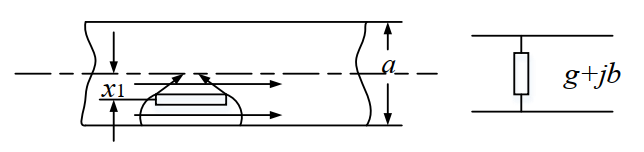
\includegraphics[height=.1\textheight]{./img/原理2.2.3a.png}
        \caption{宽边纵缝及其等效电路}
        \label{fig_principle_2.2.3a}
    \end{subfigure}\\
    \begin{subfigure}{.5\textwidth}
        \centering
        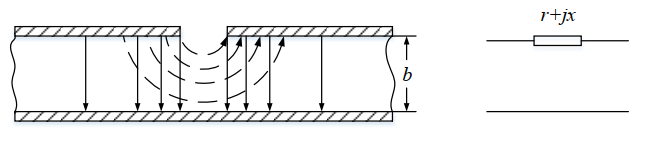
\includegraphics[height=.1\textheight]{./img/原理2.2.3b.png}
        \caption{窄边横缝及其等效电路}
        \label{fig_principle_2.2.3b}
    \end{subfigure}\\
    \begin{subfigure}{.5\textwidth}
        \centering
        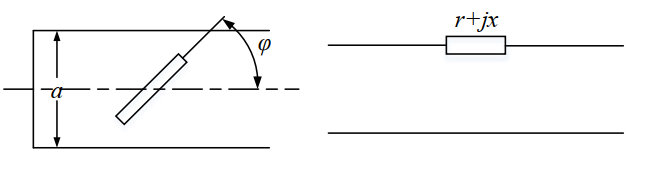
\includegraphics[height=.1\textheight]{./img/原理2.2.3c.png}
        \caption{宽边中心斜缝及其等效电路}
        \label{fig_principle_2.2.3c}
    \end{subfigure}\\
    \begin{subfigure}{.5\textwidth}
        \centering
        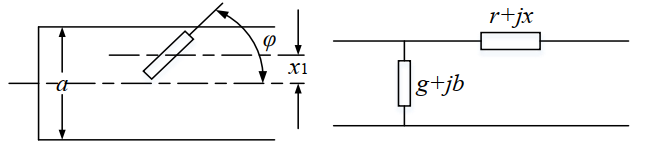
\includegraphics[height=.1\textheight]{./img/原理2.2.3d.png}
        \caption{宽边斜缝及其等效电路}
        \label{fig_principle_2.2.3d}
    \end{subfigure}\\
    \begin{subfigure}{.5\textwidth}
        \centering
        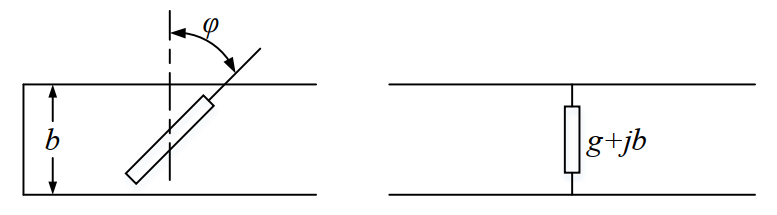
\includegraphics[height=.1\textheight]{./img/原理2.2.3e.png}
        \caption{窄边斜缝及其等效电路}
        \label{fig_principle_2.2.3e} 
    \end{subfigure}
    \caption{波导缝隙形式及其等效电路示意图}
    \label{fig_principle_2.2.3}
\end{figure}

    1.宽边纵缝[见图2.5 a)]：
\begin{equation}
    g = g_1 \sin^2\left(\frac{\pi x_1}{a}\right), \quad g_1 = 2.09 \frac{a \lambda_g}{b \lambda} \cos^2\left(\frac{\pi \lambda}{2 \lambda_g}\right)
\end{equation}
    
    2.宽边横缝[见图2.5 b)]：
\begin{equation}
    r = 0.523 \left( \frac{\lambda_g}{\lambda} \right)^2 \left( \frac{\lambda^2}{ab} \right) \cos^2\left(\frac{\pi \lambda}{4a}\right) \cos^2\left(\frac{\pi x_1}{a}\right)
\end{equation}

    3.宽边对称斜缝[见图2.5 c)]：
\begin{equation}
    r = 0.131 \frac{\lambda^3}{\lambda_g ab} \left[ f_1(\phi) \sin \phi + \frac{\lambda_g}{2a} f_2(\phi) \cos \phi\right]^2 
\end{equation}
    如果$\phi$并不大，可以进行近似求解：
\begin{equation}
    r = 0.542 \frac{\lambda_g \lambda}{ab} \left[ \frac{\beta}{2} \sin\left(\frac{\pi \lambda}{2\lambda_g}\right) - \frac{4a^2}{\lambda_g \lambda} \cos\left(\frac{\pi \lambda}{2\lambda_g}\right) \right] \phi^2
\end{equation}
    式中$\phi$ 为弧度制。
    4.宽边偏置斜缝[见图2.5 d)]：
    如果$x_1$、$\phi$均不大时，有：
\begin{equation}
    g = 0.131 \,\frac{\lambda}{\lambda_g}\,\frac{\lambda^2}{ab}\left(a_1^2 + b_1^2\right)
\end{equation}
\begin{equation}
    a_1 = \sin\left(\frac{\pi x_1}{a}\right)
    \left[
    f_2(\phi)\sin\phi+\frac{\lambda_g}{2a} f_1(\phi)\cos\phi
    \right]
\end{equation}
\begin{equation}
    b_1 = \cos\left(\frac{\pi x_1}{a}\right)
    \left[
    f_1(\phi)\sin\phi+\frac{\lambda_g}{2a} f_2(\phi)\cos\phi
    \right]
\end{equation}
    5.窄边斜缝[见图2.2 e)]：
\begin{equation}
    g = 0.131 \,\frac{\lambda^3 \lambda_g}{a^3 b}
    \left[
    \sin\phi \;
    \frac{\cos\!\left(\frac{\pi\lambda}{2\lambda_g}\sin\phi\right)}
    {1-\left(\frac{\lambda}{\lambda_g}\sin\phi\right)^2}
    \right]^2
\end{equation}
    如果$\phi$≤15°，则：
\begin{equation}
    g = A_1 \sin^2\phi \, \qquad
    A_1 = \frac{30}{73.1 \pi}\,\frac{\lambda^3 \lambda_g}{a^3 b}
\end{equation}
    虽然上文所述皆为精确的求解方法，但各自都有适用的前提条件。当互耦效应可以忽略不计时，这些方法均能直接应用；而在互耦效应不可忽视或其他复杂条件下，不同学者通过一系列研究，已针对不同情况提出了相应的求解思路。



\subsection{缝隙间的互耦}
    缝隙阵列天线由多个按特定规律排布的缝隙单元构成。由于相邻缝隙之间的间距通常不满足远大于波长的条件，它们之间的相互影响在阵列天线的设计中不可忽略。在低副瓣或极低副瓣天线的设计过程中，若忽略互耦效应，而直接采用孤立
缝隙的电参数进行设计，会导致天线口径面上的幅度分布与相位分布恶化。此外，当两个缝隙相距很近时，彼此的场分布会产生干扰，各自的阻抗相对于孤立状态也会发生变化。这些因素都会使天线输入端的匹配条件恶化，从而严重影响天线的整体性能。

\subsubsection{缝隙间互耦阻抗的等效电路和计算方法}
    波导缝隙阵列的一段如图2.6 a)所示
\begin{figure}[htb!]
    \centering
    \begin{subfigure}{.6\textwidth}
        \centering
        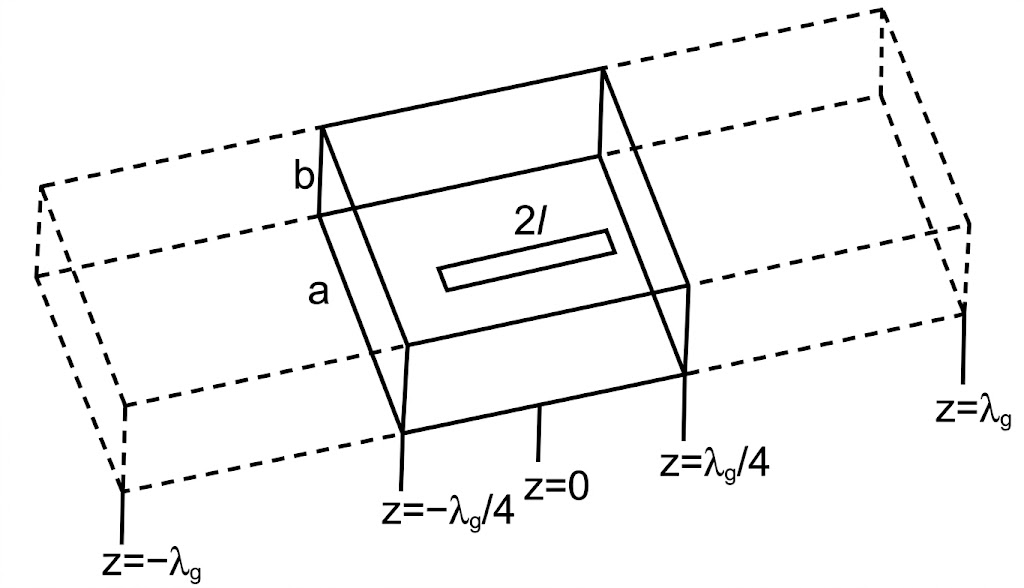
\includegraphics[height=.15\textheight]{./img/原理2.3.1a.jpg}
        \caption{单缝隙示意图}
        \label{fig_principle_2.3.1a} 
    \end{subfigure}
    \\
    \begin{subfigure}{.6\textwidth}
        \centering
        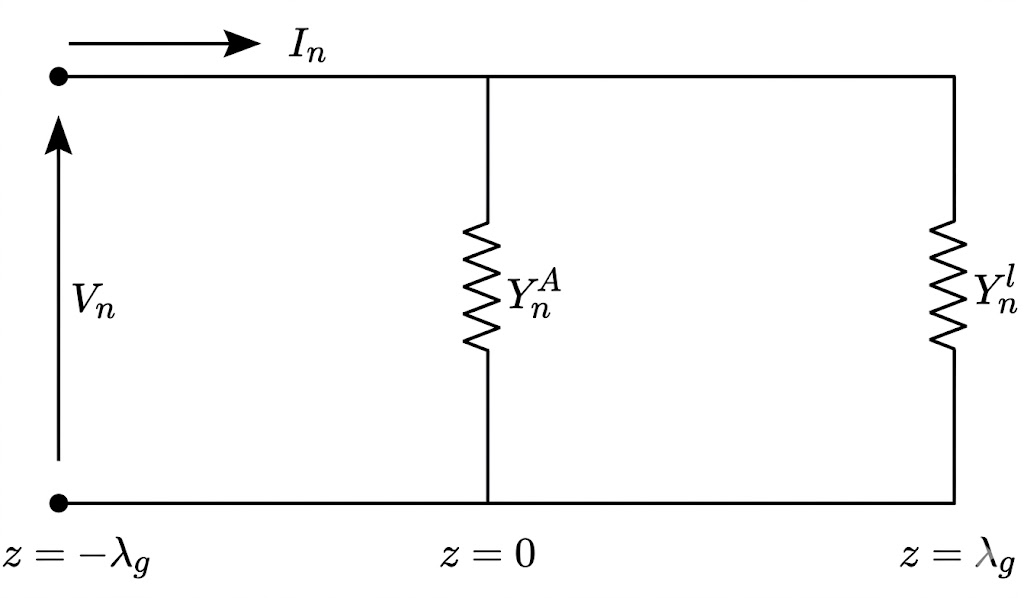
\includegraphics[height=.15\textheight]{./img/原理2.3.1b.jpg}
        \caption{等效电路}
        \label{fig_principle_2.3.1b}
    \end{subfigure}
    \caption{波导缝隙形式及其等效电路示意图}
    \label{fig_principle_2.3.1}
\end{figure}
    其中$\lambda_g$表示波导波长。假设该缝隙为阵列的第n个缝隙，缝隙中心轴线偏离波导宽面轴线的距离为$x_n$，其等效电路如图2.6 b)所示。
该等效电路的前提条件是：
    a)、波导中只有TE$_10$波传播；
    
    b)、激励源位于\(z=-\lambda_g\)处，即激励源到缝隙的距离为四分之三波长；$Y_n^A$为第n个缝隙的有源导纳，则有\supercite{25}:
\begin{equation}
    \frac{Y_n^A}{G_0} = \frac{1}{Z_n^A / 73} 
    \left\{ 
        \frac{4(a/b)}{0.61\pi(\beta/k)} [\cos(\beta l_n) - \cos(k l_n)]^2 \sin^2\left(\frac{\pi x_n}{a}\right) 
    \right\}
\end{equation}
    式中，$Z_n^A$是第n个缝隙的等效振子的有源阻抗；
\begin{equation}
    Z_n^A = Z_n + Z_n^L + \sum_{m=1}^n \frac{I_m}{I_n} Z_{mn}
\end{equation}
    式中，$Z_n$是第n个等效振子的自阻抗,$Z_n^L$是第 个等效负载阻抗；$Z_mn$是耦合阻抗；把$Y_n^A$分成两部分可以得到\supercite{4}:
\begin{equation}
    \frac{Y_n}{G_0} = 
    \frac{\frac{4(a/b)}{0.61\pi(\beta/k)} \left[ \cos(\beta l_n) - \cos(kl_n) \right]^2 \sin^2\left(\frac{\pi x_n}{a}\right)}
    {\left(\frac{Z_{mn}}{73}\right) - \sum_{m=1}^N \frac{\left(\frac{Z_{mn}}{73}\right)^2}{\left(\frac{Z_{mm}}{73}\right)}}
\end{equation}

\begin{equation}
    \frac{Y_{mn}}{G_0} = -\frac{Z_{mn}}{Z_{mm}} \cdot \frac{\left[ \cos(\beta l_n) - \cos(kl_n) \right] \sin\left(\frac{\pi x_m}{a}\right)}{\left[ \cos(\beta l_n) - \cos(kl_n) \right] \sin\left(\frac{\pi x_n}{a}\right)}
\end{equation}
    由上式可推出：
\begin{equation}
    \frac{Y^2_{mn}}{Y_m Y_n} = \frac{Z^2_{mn}}{Z_m Z_n}
\end{equation}
    由式(2.37)~(2.41)可以看出，缝隙的耦合阻抗可以通过缝隙的等效振子的耦合阻抗计算得出。

\subsubsection{振子耦合阻抗}
    当两个振子紧密排列时，辐射场之间的相互耦合会导致各自阻抗发生变化，进而改变电流的幅值与方向，最终影响天线的方向性。对于天线的耦合问题，通常采用阻抗模型进行描述，常用的分析方法包括感应电动势法和散射矩阵法\supercite{21}\supercite{22}\supercite{23}。
    设两个振子的相对位置如图2.7 a)所示，$L_1$、$L_2$分别是主振子h和从振子的长度，$x'y'z'$是以振子为中心从原点建立的从坐标系，$y_0$、$z_0$是它到主坐标系的位移量。$\theta$是从振子与$z$'轴之间的夹角，$\phi$是从振子与$x$'轴之间的夹角。根据阻抗定义有下式：
\begin{equation}
    Z_{21}=-\frac{V_{21}}{I_1}
\end{equation}
    式中，$V_{21}$是从振子在主振子上的感应电动势总和。
\begin{figure}[htb!]
    \centering
    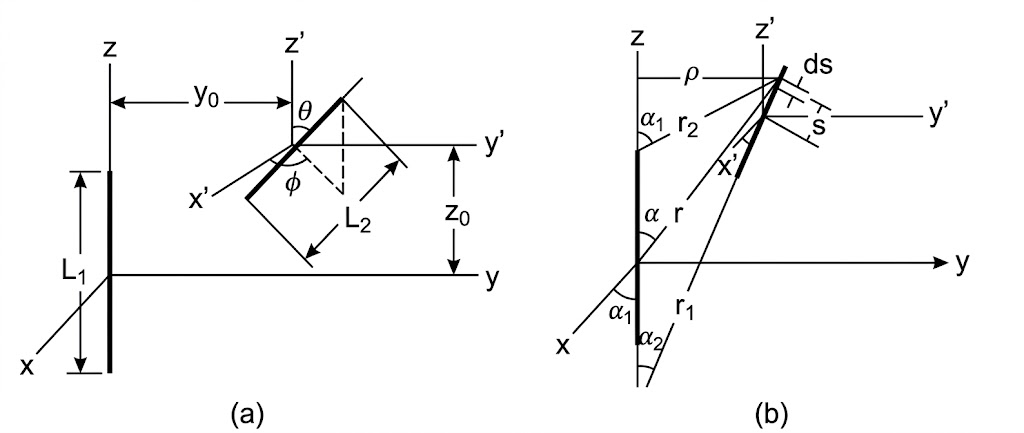
\includegraphics[width=.7\textwidth]{img/原理2.3.2.jpg}
    \caption{两振子相对位置}
    \label{fig_principle_2.3.2}
\end{figure}
\begin{equation}
    E_z = j30I_1 \left[ 2 \frac{e^{-jkR_0}}{R_0} \cos\left(\frac{kL_1}{2}\right) - \frac{e^{-jkR_1}}{R_1} - \frac{e^{-jkR_2}}{R_2} \right]
\end{equation}

\begin{equation}
    E_\rho = \frac{j30I_1}{\rho} \left[ e^{-jkR_1} \cos\alpha_1 + e^{-jkR_2} \cos\alpha_2 - 2\cos\left(\frac{kL_1}{2}\right)e^{-jkR_0}\cos\alpha \right]
\end{equation}
    式中，$I_1$为主振子的电流幅值。将上式转换到直角坐标系下有：
\begin{equation}
    E_x=E_{\rho}\frac{S_x}{\rho}
\end{equation}
\begin{equation}
    E_y=E_{\rho}\frac{y_0+S_y}{\rho}
\end{equation}
\begin{equation}
    E_z=E_z
\end{equation}
\begin{equation}
    E_{21} = \frac{\bar{E} \cdot \bar{S}}{S} = \frac{E_x S_x + E_y S_y + E_z S_z}{S}
\end{equation}
    把式(2.45)~(2.47)代入式(2.48)得:
\begin{equation}
    E_{21} = \frac{ \frac{E_{x}^{2} + S_{y}y_{0} + S_{y}^{2}}{\rho} + E_{z}S_{z} }{S}
\end{equation}
